\section{Resultater}
\label{ch:Resultater}
I dette afsnit samles der op på resultaterne gruppen har opnået gennem projektforløbet. Her vil der blive beskrevet resultater for de enkelte moduler gruppen har implementeret. Til sidst bliver der knyttet en kommentar til det samlede resultat. Der vil i afsnittet blive henvist til testresultater dokumenteret i dokumentationsdokumenterne, henholdsvis \textit{Enhedstest}, \textit{Integrationstest} og \textit{Accepttest}.

\subsection{Kontrolinterfacet}
Kontrolinterfacet er fuldt implementeret og har opfyldt alle enhedstests for modulet. TCP- og UART-kommunikationen er udviklet i Qt med API'er specifikke for Qt. Der er dog flere steder hvor der godt kunne ske forbedringer (se afsnit \ref{ch:Forbedringer}). Slutresultatet er et tilfredsstillende resultat med tanke på at arbejdsbyrden er løftet som en enkeltmandsopgave.\\

\subsection{Database og webinterface}
Database og Webinterfacet er fuldt implementeret. I database-modulet er serveren fuldt kørende og har en stabil forbindelse med Kontrolinterfacet via TCP. Serveren er i stand til at gemme alle data til en tekstfil men at gemme direkte til MySQL databasen blev aldrig implementeret, da der opstod problemer med MySQL driver og header.\\
Webinterfacet er fuldt implementeret og ved opstart fungerer indtastningen af brugeradgangskoden korrekt med undtagelse ved forkert indtastet adgangskode. Her bliver brugeren ikke bedt om at taste nyt password, men får i stedet en blank side. Brugeren har dog ikke adgang til data.

\subsection{Styringsmodul}
Styringsmodulet er fuldt implementeret, men ikke finjusteret. Forbindelsen til Kontrolinterfacet er fuldt funktionel. Forbindelsen til VBTE virker 95\% af tiden. Automatisk hældningsregulering er implementeret, men da niveaumålinger ikke modtages fra Vandballasttankenhederne er det ikke muligt at tømme tankene inden der fyldes i den anden tank. Prototypen af modulet er monteret med 7 LED's der bruges til fejlfinding. Prototypen er også lagt ud på print med indeholdende levelkonvertering og I2C pull-up modstande.

\subsection{Vandballasttankenhederne}
VBTE-modulet nåede aldrig at komme til at fungere optimalt. Efter at have implementeret ultralydsafstandsensoren  og undersøgt/tweaket på parametrene viste det sig at det ikke fungerede ret godt over længere afstande (i hvert fald i dette design). Dette kan skyldes at der blev anvendt for lav en spænding over transduceren eller at der skulle filtreres på det modtagede signal så det kunne forstærkes mere op. Under kontrollerede forhold i laboratoriet lykkedes det at få flotte detektioner på ultralydsafstandssensoren som kan ses på \textit{figur \ref{res:ultraresultater}}.
\begin{figure}[H]
\centering
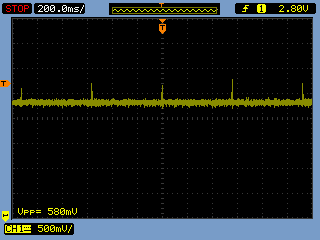
\includegraphics[width = .5\textwidth]{billeder/mixer2}
\caption{Detektioner af ultralydsafstandssensoren med faste intervaller.}
\label{res:ultraresultater}
\end{figure}
Derudover virkede I2C-delen, dog med fejl på data i enkelte transmissioner. Det vides ikke om det er et normalt problem ved I2C eller om det havde noget at gøre med vores system. Til sidst er der udlagt print til VBTE'en, en 2x16 LCD skærm til test samt dipswitches og knap til at skifte I2C-adresse mens systemet kører. 

\subsection{Strømforsyning}
Strømforsyningen er fuldt implementeret. I testen er der blevet brugt effektmodstande som lod, en laboratoriestrømforsyning og et voltmeter. Enhedstesten er blevet godkendt. Vitale dele på strømforsyningen bliver dog noget varme ved fuld load på udgangen, men da det med stor sandsynlighed sjældent vil ske, ses det ikke som et problem. Strømforsyningen er implementeret med Styringsmodulet og Vandballasttankenhederne. Derudover er der udlagt et print med 12V- og 5V-forsyning.

\subsection{Samlede resultat og vurdering af resultater}
\label{ch:samlresultat}
Til de samlede resultater har gruppen udarbejdet en tabel der viser hvordan resultatet af testforløbet fra enhedstest til accepttest. For detaljer om den enkelte test henvises til \textit{Enhedstest}, \textit{Integrationstest} og \textit{Accepttest}. Testresultaterne er opdelt i fire katagorier som angivet i tabellen:
\begin{table}[H]
\centering
\begin{tabular}{cccc}
\hline
Godkendt 	& Delvist godkendt 	& Ikke godkendt & Ikke testet \\
\cmidrule(r){1-1} \cmidrule(r){2-2} \cmidrule(r){3-3} \cmidrule(r){4-4}
$\surd$		& $\times$		& $\div$ & $\diamond$	\\\hline
\end{tabular}
\caption{Testgodkendelseskategorier}
\end{table}
\begin{table}[H]
\centering
\begin{tabular}{llllllll}
\hline
\multicolumn{1}{c}{Test} & \multicolumn{7}{c}{Test case ID}\\
\cmidrule(r){1-1} \cmidrule(r){2-8} 
\textbf{Enhedstest software} & 1 & 2 & 3 & 4 & 5 & 6 & 7\\
\hline
\phantom{mm}Kontrolinterface& $\surd$ & $\surd$ & $\surd$ & $\surd$ & $\surd$ \\
\phantom{mm}Database  		& $\surd$ & $\surd$ & $\surd$ & $\surd$ & $\surd$ \\
\phantom{mm}Styringsmodulet	& $\surd$ & $\surd$ & $\surd$ & $\surd$ & $\surd$ &  $\surd$ & $\surd$\\
\phantom{mm}VBTE  			& $\surd$ & $\surd$ & $\surd$ & $\surd$ & $\surd$ \\ 
\textbf{Enhedstest hardware} \\
\hline
\phantom{mm}Styringsmodul	& $\surd$ & $\surd$\\
\phantom{mm}VBTE  			& $\surd$ & $\surd$ & $\times$ \\ 
\phantom{mm}Strømforsyning 	& $\surd$ & $\surd$ & $\surd$\\
\hline
\textbf{Integrationstest} 	& $\surd$ & $\surd$ & $\surd$ & $\surd$ & $\surd$ & $\surd$\\
\textbf{Accepttest} 		& $\surd$ & $\times$ & $\times$ & $\surd$ & $\surd$ & $\surd$\\
\hline
\end{tabular}
\caption{Samlet tabel med alle resultater}
\label{table:alle test samlet}
\end{table}
Som tabellen illustrerer er der blevet implementeret en masse funktionaliteter, som er blevet godkendt gennem enhedstest. Dog var der problemer med afstandsmåling på VBTE og denne testcase kunne derfor kun delvist godkendes.\\
Integrationen af systemets enheder er blevet godkendt.\\
Grundet problemer med afstandmåling på VBTE kan Accepttest case 2 og 3 kun delvist godkendes.\\